
% --- quiz1 ---
\element{essai}{
  \begin{questionmult}{q:quiz1}
  What are the signal characteristics and the initial objectives described in the $\text{Lab}$ on digital filtering?
    \begin{choices}
      \correctchoice{The studied signal is corrupted by a slow drift ($\text{drift}$) of its mean value, a common problem in sensor measurements.}
      %answer: The signal is corrupted by a slow drift, which is a common problem with sensor measurements.
      %tip: Check the initial description of the signal.
      \correctchoice{One of the objectives of the $\text{Lab}$ is to design a filter to remove this slow drift.}
      %answer: A first filter will be designed in order to remove this drift.
      %tip: The first filtering objective is the removal of the drift.
      \wrongchoice{The sampling frequency specified for the signal analysis is $\text{Fs}=800 \text{ Hz}$.}
      %answer: The specified sampling frequency is $\text{Fs}=8000 \text{ Hz}$.
      %tip: Check the numerical value of the sampling frequency.
      \wrongchoice{The signal is periodic with a period of about $40 \text{ Hz}$ in the frequency domain.}
      %answer: The signal is periodic with a period of about 40 in the time domain, and not in frequencies.
      %tip: The period is a time measurement, not a frequency measurement.
    \end{choices}
\end{questionmult}
}

% --- quiz2 ---
\element{nocategory}{
  \begin{questionmult}{q:quiz2}
  According to the time and frequency analysis of signal $\text{x}$, which observations are correct?
    \begin{choices}
      \correctchoice{The time signal $\text{x}$ is approximately periodic with a period of about $40$ samples.}
      %answer: We observe an approximately periodic time series, with a period of about 40.
      %tip: The analysis of the signal in the time domain is described.
      \correctchoice{The Fourier Transform ($\text{FT}$) of the signal consists of a series of regularly spaced spectral lines, indicating a periodic underlying signal.}
      %answer: We see that the Fourier Transform consists of a series of regularly spaced spectral lines, which is an indication that the underlying signal is periodic.
      %tip: The appearance of the $\text{FT}$ is related to the periodicity of the signal.
      \wrongchoice{The $\text{FT}$ of the signal shows a spectral peak spacing of $0.025$ in non-normalized frequencies (Hertz).}
      %answer: The peaks are spaced by $0.025$ in normalized frequencies.
      %tip: The spacing is given in normalized frequencies.
      \wrongchoice{The analysis of the $\text{FT}$ shows only the slow drift component without any other spectral lines.}
      %answer: The $\text{FT}$ shows a series of regularly spaced spectral lines and a slow drift (average value).
      %tip: The signal contains several frequency components.
    \end{choices}
\end{questionmult}
}

% --- quiz54 is a template - Generating random values ---
% a = -1.1005063209227404
% b = -2.4942790823787475
\element{nocategory}{
  \begin{question}{q:quiz54}
  This is a numeric question where you must calculate the sum and difference of -1.1005 and -2.4943
  \AMCNumericChoices{-3.5948}{digits=3,decimals=2,sign=true}
  \AMCNumericChoices{1.3938}{digits=3,decimals=2,sign=true}
\end{question}
}

% --- quiz59 ---
\element{nocategory}{
  \begin{question}{q:quiz59}
  Please enter the mean and standard deviation values of the time series above
  \AMCNumericChoices{0.0}{digits=3,decimals=2,sign=true}
  \AMCNumericChoices{1.0}{digits=3,decimals=2,sign=true}
\end{question}
}

% --- quiz63 is a template - Generating random values ---
% n = 4
\element{nocategory}{
  \begin{question}{q:quiz63}
  What is the derivative of $x^n$, with n=4, that is  $x^{4}$,
    \begin{choices}
      \correctchoice{The derivative is $4 x^{3}$}
      %answer: 
      %tip: 
      \wrongchoice{The derivative is $\frac{1}{4} x^{4}$}
      %answer: 
      %tip: 
      \wrongchoice{The derivative is $\frac 1{3} x^{3}$}
      %answer: 
      %tip: 
      \wrongchoice{The derivative is $3 x^{3}$}
      %answer: 
      %tip: 
    \end{choices}
\end{question}
}

% --- quiz79 is a template - Generating random values ---
% FN = 3
% FP = 5
% TN = 15
% TP = 22
\element{test}{
  \begin{question}{q:quiz79}
  Consider the following \emph{confusion matrix}:
{\def\LTcaptype{none} % do not increment counter
\begin{longtable}[]{@{}lll@{}}
\toprule\noalign{}
True/Predict & 0 & 1 \\
\midrule\noalign{}
\endhead
\bottomrule\noalign{}
\endlastfoot
0 & 15 & 5 \\
1 & 3 & 22 \\
\end{longtable}
}
  \AMCNumericChoices{0.88}{digits=3,decimals=2,sign=true}
  \AMCNumericChoices{0.822}{digits=3,decimals=2,sign=true}
\end{question}
}

% --- quiz81 is a template - Generating random values ---
% w0 = 0.83651883399106
% w1 = 0.7321965285932113
% x = 0.09426838472463968
\element{test}{
  \begin{question}{q:quiz81}
  Consider a scatter plot such as the one shown in the figure
\begin{figure}
\centering
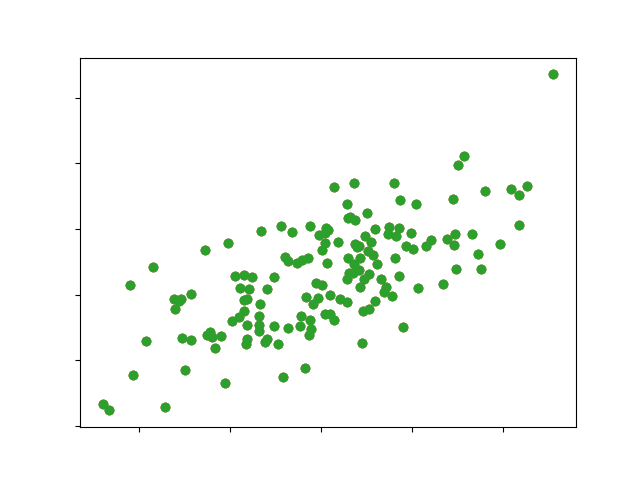
\includegraphics[width=0.38\linewidth,height=\textheight,keepaspectratio,alt={Scatter plot}]{./Figure_1.png}
\caption{Scatter plot}
\end{figure}
We perform a linear regression \texttt{reg}, which yields - \texttt{reg.intercept\_} = 0.837 and - \texttt{reg.coef\_} = 0.732. For a new observation x = 0.094, what would be the value predicted by the model?
  \AMCNumericChoices{0.906}{digits=3,decimals=2,sign=true}
\end{question}
}

% --- quiz82 is a template - Generating random values ---
% a = -1.3421846845486378
% b = -0.24600000286920742
% x = 0.42657556159361454
% x2 = 1.1913600283956391
\element{test}{
  \begin{question}{q:quiz82}
  Consider the simple regression  model 
$$
y = \alpha x + \beta
$$
with $\alpha={-1.342}$ and $\beta={-0.246}$
    \begin{choices}
      \wrongchoice{For x=1.191, the prediction is -1.635}
      %answer: Prediction is simply computed by $y = \alpha x + \beta$ 
      %tip: 
      \correctchoice{For x=0.427, the prediction is -0.819  
}
      %answer: Prediction is simply computed by $y = \alpha x + \beta$
      %tip: 
      \wrongchoice{The slope is positive}
      %answer: The slope is actually not positive, since it is equal to $\alpha$=-1.342
      %tip: 
    \end{choices}
\end{question}
}